The application of the UR5 known as \productname{} is designed to reduce the cost of owning a business oriented around preparing food. With the increase in demand towards a higher minimum wage, many businesses will be seeking options to save money.

\subsection{Purpose and Use}
\productname{} will be able to prepare food (specifically hamburgers) to serve to a consumer. You will be able to queue up requests and receive the food.  

\subsection{Intended Audience}
The target audience for \productname{} are restaurant owners (more specifically ones that run chain restaurants), as \productname{} will allow them to save money on hiring workers.

This will allow owners to save money, worry less about payroll taxes, and serve quality food at a lower cost.

\begin{figure}[h!]
	\centering
   	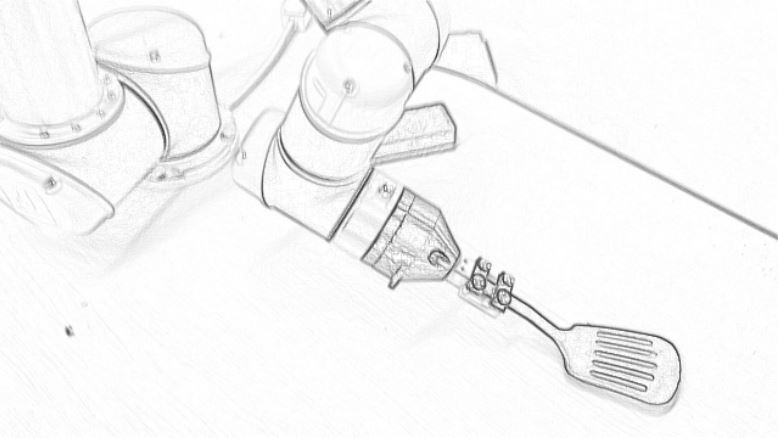
\includegraphics[width=0.60\textwidth]{images/test_image}
    \caption{X conceptual drawing}
\end{figure}
